% 2008 年山东卷文科第 19 题：四棱锥 P-ABCD，平面 PAD⊥平面 ABCD，AB∥DC，
%   △PAD 为等边三角形，BD=2AD=8，AB=2DC=4√5，M 为 PC 上一点。
% 来源 PDF：gaokaomath-src/普通高考/2008/2008山东文.pdf
% SHA-256：479a9abc0fe5954c5b717d8eb0f649966c1cee3cfabdab00f10cc5834668fd6f
% 原页：2008山东文.pdf 第 2 页（A3 三栏）第 1 栏，书页码 474。
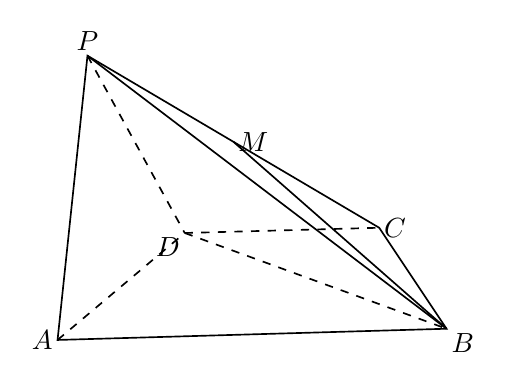
\begin{tikzpicture}[scale=0.95, semithick,
  every node/.style={inner sep=1.5pt}]
  \coordinate (A) at (0.70,0.60);
  \coordinate (B) at (5.90,0.75);
  \coordinate (C) at (5.00,2.10);
  \coordinate (D) at (2.40,2.03);
  \coordinate (P) at (1.10,4.40);
  \coordinate (M) at (3.05,3.25);

  % 可见棱
  \draw (A) -- (B) -- (C) -- (P) -- cycle;
  \draw (P) -- (B);
  \draw (M) -- (B);

  % 被遮挡的棱
  \draw[dashed] (P) -- (D);
  \draw[dashed] (A) -- (D) -- (C);
  \draw[dashed] (D) -- (B);

  \node[above] at (P) {$P$};
  \node[left] at (A) {$A$};
  \node[below right] at (B) {$B$};
  \node[right] at (C) {$C$};
  \node[below left] at (D) {$D$};
  \node[right] at (M) {$M$};
\end{tikzpicture}
